



\section{Convex Optimization Examples}
\subsection{Unconstrained Optimization: Linear Regression}

Given data points $x^1, \dots, x^N \in \R^d$ and out values $y^i \in \R$, we want to find a linear function $y = \beta \cdot x$ that best approximates $x^i \cdot \beta \approx y^i$.  For example, the data could $x = (\text{time})$ and the output could be $y = \text{position}$.  


\includefiguresource[Line derived through linear regression.][scale = 1]{tikz/linear-regression.pdf}

%\begin{figure}[H]
%\begin{center}
%\includegraphicstatic[scale = 1]{LinearRegression.pdf}\footnotemark
%\en
%d{center}
%\end{figure}
%\footnotetext{\url{https://latexdraw.com/linear-regression-in-latex-using-tikz/}}


As is standard, we choose the error (or "loss") from each data point as the squared error.  Hence, we can model this as the optimization problem:
\begin{align}
\label{eq:least-squares}
\min_{\beta \in \R^d} & \sum_{i=1}^N (x^i \cdot \beta - y^i)^2.
\end{align}
Equivalently, we could write this as 
\[
\min_{\mathbf{\beta}} \|X \mathbf{\beta} -\mathbf{y}\|_2,
\]
where 
$$X = 
\begin{bmatrix}
\mathbf{x}^1\\
\vdots \\
\mathbf{x}^N
\end{bmatrix}
= 
\begin{bmatrix}
x^1_1 & x^1_2 & \dots & x^1_d\\
\vdots \\
x^N_1 & x^N_2 & \dots & x^N_d
\end{bmatrix}
$$

This problem has a nice closed form solution.  We will derive this solution, and then in a later section discuss why using this solution might be too  slow to compute on large data sets.  In particular, the solution comes as a system of linear equations.  But when $N$ is really large, we may not have time to solve this system, so an alternative is to use decent methods, discussed later in this chapter.

\begin{theorem}{Linear Regression Solution}{}
The optimal solution to \eqref{eq:least-squares} is 
\begin{equation}
\mathbf{\beta}^* = (X^\top X)^{-1} X^\top \mathbf{y}.
\end{equation}
\end{theorem}
\begin{proof}
We rewrite the objective function in matrix form as
\[
L(\mathbf{\beta}) = \sum_{i=1}^N (\mathbf{x}^i \cdot \mathbf{\beta} - y_i)^2 = (X\beta - \mathbf{y})^\top (X\mathbf{\beta} - \mathbf{y})
= \beta^\top X^\top X \mathbf{\beta} - 2\mathbf{y}^\top X \mathbf{\beta} + \mathbf{y}^\top \mathbf{y}.
\]
Observe that the obective is a sum of squares of linear terms, so it is a convex function!  Thus, to find the value of \(\mathbf{\beta}\) that minimizes \(L(\mathbf{\beta})\) we solve for setting the gradient equal to 0:
\[
\nabla L(\mathbf{\beta}) = 2X^\top X \mathbf{\beta} - 2X^\top \mathbf{y} = 0  \ \ \ \Rightarrow \ \ \ 
X^\top X \beta = X^\top \mathbf{y}
\ \ \ \Rightarrow \ \ \
\beta = (X^\top X)^{-1} X^\top \mathbf{y}
\]
This completes the proof.

\textit{Note:} The solution assumes that \(X^\top X\) is invertible. If it's not, then the least squares solution may not be unique.
\end{proof}



\begin{examplewithcode}{Predicting Manufacturing Costs}{}

Consider a manufacturing facility that produces a variety of parts for industrial machinery. The management wants to predict the production cost of a new part based on various factors such as material costs, labor hours, machine hours, and energy consumption.

\paragraph{Data Collection}

The first step is to collect historical data of the manufactured parts including:

\begin{itemize}
  \item Material costs (\$)
  \item Labor hours
  \item Machine hours
  \item Energy consumption (kWh)
  \item Production cost (\$)
\end{itemize}

\begin{table}[ht]
\centering
\begin{tabular}{ccccc}
\hline
\textbf{Material Cost (\$)} & \textbf{Labor Hours} & \textbf{Machine Hours} & \textbf{Energy Consumption (kWh)} & \textbf{Production Cost (\$)} \\ \hline
1500                       & 35                   & 30                     & 500                               & 8000                         \\
2000                       & 40                   & 25                     & 550                               & 8500                         \\
2500                       & 45                   & 50                     & 600                               & 9000                         \\
3000                       & 30                   & 45                     & 650                               & 9500                         \\
3500                       & 50                   & 35                     & 700                               & 10000                        \\
4000                       & 55                   & 55                     & 750                               & 10500                        \\
4500                       & 65                   & 65                     & 800                               & 11000                        \\
1800                       & 25                   & 20                     & 450                               & 7700                         \\
2200                       & 22                   & 30                     & 500                               & 7900                         \\
3000                       & 48                   & 40                     & 670                               & 9900                         \\
3200                       & 50                   & 42                     & 680                               & 10100                        \\
2800                       & 36                   & 38                     & 620                               & 9300                         \\
2300                       & 32                   & 28                     & 540                               & 8100                         \\ \hline
\end{tabular}
\caption{Sample data for predicting manufacturing costs}
\label{table:manufacturing_costs}
\end{table}


\paragraph{Model Development}

Using the collected data, a linear regression model can be constructed where the production cost (\$) is the dependent variable, and the material costs, labor hours, machine hours, and energy consumption are the independent variables.

\paragraph{Statistical Analysis}

The linear regression analysis will result in an equation of the form:

\begin{equation}
\text{Production Cost} = \beta_0 + \beta_1 \times \text{Material Cost} + \beta_2 \times \text{Labor Hours} + \beta_3 \times \text{Machine Hours} + \beta_4 \times \text{Energy Consumption} + \epsilon
\end{equation}

where $\beta_0$ is the y-intercept, $\beta_1, \beta_2, \beta_3,$ and $\beta_4$ are the coefficients representing the impact of each independent variable on the production cost, and $\epsilon$ is the error term.

\paragraph{Decision Making}

By fitting the linear regression model to the data, the facility can predict the cost of producing new parts based on the estimated regression coefficients. This model will help in pricing decisions, cost-saving strategies, and optimizing the use of resources.

\paragraph{Visualization}

A scatter plot with a fitted regression line can help visualize the relationship between the production cost and any of the independent variables, such as labor hours:

\begin{figure}[h!]
  \centering
  %\includegraphics[width=0.8\textwidth]{regression-plot.png}
  \caption{Scatter plot of production cost against labor hours with fitted regression line}
\end{figure}


\end{examplewithcode}

%
%
%\section*{Regression Problems} % ==============================================
%
%A major use of the conjugate gradient method is solving linear least squares problems.
%Recall that a least squares problem can be formulated as an optimization problem:
%\[
%\x^* = \min_\x \|A\x -\textbf{ b}\|_2,
%\]
%where $A$ is an $m \times n$ matrix with full column rank, $\x \in \mathbb{R}^n$, and $\b \in \mathbb{R}^m$. The solution can
%be calculated analytically, and is given by
%\[
%\x^* = (A\trp A)^{-1}A\trp \b.
%\]
%In other words, the minimizer solves the linear system
%\begin{equation}
%A\trp A\x = A\trp \b.
%\label{eq:ls}
%\end{equation}
%Since $A$ has full column rank, it is invertible, $A\trp A$ is positive definite, and for any non-zero vector $\textbf{z}$, $A\textbf{z}\neq 0$.
%Therefore, $\textbf{z}\trp A\trp A\textbf{z} = \Vert A\textbf{z} \Vert^2 > 0$.
%As $A\trp A$ is positive definite, conjugate gradient can be used to solve Equation \ref{eq:ls}.
%
%Linear least squares is the mathematical underpinning of \emph{linear regression}.
%Linear regression involves a set of real-valued data points \{$y_1,\ldots, y_m\}$, where each
%$y_i$ is paired with a corresponding set of predictor variables $\{x_{i,1}, x_{i,2}, \ldots, x_{i,n}\}$ with $n < m$.
%The linear regression model posits that
%\[
%y_i = \beta_0 + \beta_1 x_{i,1} + \beta_2 x_{i,2} + \cdots + \beta_n x_{i,n} + \epsilon_i
%\]
%for $i = 1, 2, \ldots, m$.
%The real numbers $\beta_0,\ldots,\beta_n$ are known as the parameters of the model, and the $\epsilon_i$ are independent, normally-distributed error terms.
%The goal of linear regression is to calculate the parameters that best fit the data.
%This can be accomplished by posing the problem in terms of linear least squares.
%Define
%\[
%\b = \left[\begin{array}{c}y_1 \\ \vdots \\ y_m\end{array}\right],
%\quad
%A =
%\left[\begin{array}{ccccc}
%1 & x_{1,1} & x_{1,2} & \cdots & x_{1,n}\\
%1 & x_{2,1} & x_{2,2} & \cdots & x_{2,n}\\
%\vdots & \vdots & \vdots & \ddots & \vdots\\
%1 & x_{m,1} & x_{m,2} & \cdots & x_{m,n}
%\end{array}\right],
%\quad
%\x = \left[\begin{array}{c}
%    \beta_0 \\ \beta_1 \\ \vdots \\ \beta_n
%\end{array}\right].
%\]
%The solution $\x^* = [\beta_0^*, \beta_1^*, \ldots, \beta_n^*]\trp$ to the system $A\trp A\x = A\trp\b$ gives the parameters that best fit the data.
%These values can be understood as defining the hyperplane that best fits the data.
%
%\begin{figure}[H]
%\centering
%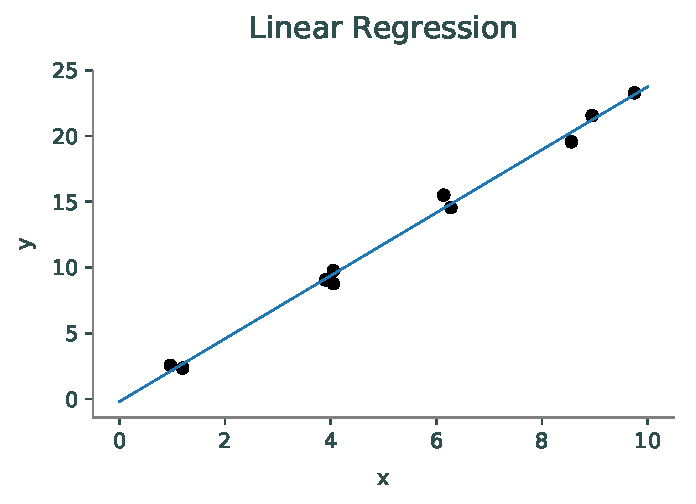
\includegraphics[width=.7\textwidth]{foundationsAppliedMathematicsLabs/Volume2/GradientMethods/figures/linregression.pdf}
%\caption{Solving the linear regression problem results in a best-fit hyperplane.}
%\label{fig:linregression}
%\end{figure}
%
%\begin{problem}{}{}
%Using your function from Problem \ref{prob:gradientmethods-linear-cg}, solve the linear regression problem specified by the data contained in the file\footnote{Source: Statistical Reference Datasets website at \url{http://www.itl.nist.gov/div898/strd/lls/data/LINKS/v-Longley.shtml}.}
%\texttt{linregression.txt}.
%This is a whitespace-delimited text file formatted so that the $i$-th row consists of $y_i, x_{i,1}, \ldots, x_{i,n}$.
%Use \li{np.loadtxt()} to load in the data and return the solution to the normal equations.
%\end{problem}

\subsection*{Logistic Regression} % -------------------------------------------

\emph{Logistic regression} is another important technique in statistical analysis and machine learning that builds off of the concepts of linear regression.
As in linear regression, there is a set of predictor variables $\{x_{i, 1}, x_{i, 2}, \dots, x_{i, n}\}_{i = 1}^{m}$ with corresponding outcome variables $\{y_i\}_{i = 1}^{m}$.
In logistic regression, the outcome variables $y_i$ are binary and can be modeled by a \emph{sigmoidal} relationship.
The value of the predicted $y_i$ can be thought of as the probability that $y_i = 1$.
In mathematical terms,
\[
\mathbb{P}(y_i = 1 \, | \, x_{i,1}, \dots, x_{i,n}) = p_i,
\]
where
\[
p_i = \frac{1}{1+\exp(-(\beta_0 + \beta_1x_{i,1} + \dots + \beta_nx_{i,n}))}.
\]
The parameters of the model are the real numbers $\beta_0, \beta_1,\dots, \beta_n$.
Note that $p_i \in (0, 1)$ regardless of the values of the predictor variables and parameters.

The probability of observing the outcome variables $y_i$ under this model, assuming they are independent, is given by
the \emph{likelihood function} $\mathcal{L}:\mathbb{R}^{n+1} \rightarrow \mathbb{R}$
\[
\mathcal{L}(\beta_0, \dots, \beta_n) = \prod_{i=1}^m p_i^{y_i}(1-p_i)^{1-y_i}.
\]
The goal of logistic regression is to find the parameters $\beta_0, \dots, \beta_k$ that maximize this likelihood function.
Thus, the problem can be written as:
\[
\max_{(\beta_0,\dots,\beta_n)}\mathcal{L}(\beta_0, \dots, \beta_n).
\]

Maximizing this function is often a numerically unstable calculation.
Thus, to make the objective function more suitable, the logarithm of the objective function may be maximized because the logarithmic function is strictly monotone increasing.
Taking the $\log$ and turning the problem into a minimization problem, the final problem is formulated as:
\[
\min_{(\beta_0,\dots,\beta_n)} - \log\mathcal{L}(\beta_0, \dots, \beta_n).
\]

A few lines of calculation reveal that this objective function can also be rewritten as
\begin{align*}
-\log\mathcal{L}(\beta_0,\dots,\beta_n) = &\sum_{i=1}^{m}\log(1+\exp(-(\beta_0 + \beta_1x_{i,1} + \dots +\beta_nx_{i,n}))) +\\
 &\sum_{i=1}^m (1- y_i)(\beta_0 + \beta_1x_{i,1} + \dots + \beta_nx_{i,n}).
\end{align*}

The values for the parameters  $\{\beta_i\}_{i = 1}^{n}$ that we obtain are known as the \emph{maximum likelihood estimate} (MLE).
To find the MLE, conjugate gradient can be used to minimize the objective function.

For a one-dimensional binary logistic regression problem, we have predictor data $\{x_i\}_{i=1}^m$ with labels $\{y_i\}_{i=1}^m$ where each $y_i \in \{0, 1\}$.
The negative log likelihood then becomes the following.
\begin{equation}
-\log\mathcal{L}(\beta_0, \beta_1) = \sum_{i=1}^m \log(1 + e^{-(\beta_0 + \beta_1 x_i)}) + (1 - y_i)(\beta_0 + \beta_1 x_i)
\label{eq:gradientmethods-negative-log-likelihood}
\end{equation}

%\begin{problem}{}{}
%Write a class for doing binary logistic regression in one dimension that implement the following methods.
%\begin{enumerate}
%\item \li{fit()}: accept an array $\x\in\mathbb{R}^n$ of data, an array $\y\in\mathbb{R}^n$ of labels ($0$s and $1$s), and an initial guess $\boldsymbol{\beta}_0\in\mathbb{R}^2$.
%Define the negative log likelihood function as given in \eqref{eq:gradientmethods-negative-log-likelihood}, then minimize it (with respect to $\boldsymbol{\beta}$) with your function from Problem \ref{prob:gradientdescent-nonlinear-cg} or \li{opt.fmin_cg()}.
%Store the resulting parameters $\beta_0$ and $\beta_1$ as attributes.
%
%\item \li{predict()}: accept a float $x\in\mathbb{R}$ and calculate
%\[\sigma(x) = \frac{1}{1 + \exp(- (\beta_0 + \beta_1 x))},\]
%where $\beta_0$ and $\beta_1$ are the optimal values calculated in \li{fit()}.
%The value $\sigma(x)$ is the probability that the observation $x$ should be assigned the label $y=1$.
%\end{enumerate}
%This class does not need an explicit constructor.
%You may assume that \li{predict()} will be called after \li{fit()}.
%\label{prob:gradientmethods-logistic-regression}
%\end{problem}

\begin{example}{Challenger damage prediction}{}
On January 28, 1986, less than two minutes into the Challenger space shuttle's 10th mission, there was a large explosion that originated from the spacecraft, killing all seven crew members and destroying the shuttle.
The investigation that followed concluded that the malfunction was caused by damage to O-rings that are used as seals for parts of the rocket engines.
There were 24 space shuttle missions before this disaster, some of which had noted some O-ring damage.
Given the data, could this disaster have been predicted?

The file \href{https://github.com/open-optimization/open-optimization-or-examples/blob/master/nonlinear-programming/challenger-data.csv}{challenger-data.csv} contains data for 23 missions (during one of the 24 missions, the engine was lost at sea).
The first column ($\x$) contains the ambient temperature, in Fahrenheit, of the shuttle launch.
The second column ($\y$) contains a binary indicator of the presence of O-ring damage (1 if O-ring damage was present, 0 otherwise).

The logistic regression is implemented in \href{https://github.com/open-optimization/open-optimization-or-examples/blob/master/nonlinear-programming/logistic-regression-challenger.ipynb}{logistic-regression-challenger.ipynb} using the python package \emph{sklearn}.

On the day on launch, the temperature was $31^\circ$F.
The predicted probability (according to this model) of O-ring damage on the day the shuttle was launched, is 0.9996.  

\begin{figure}[H]
\centering
    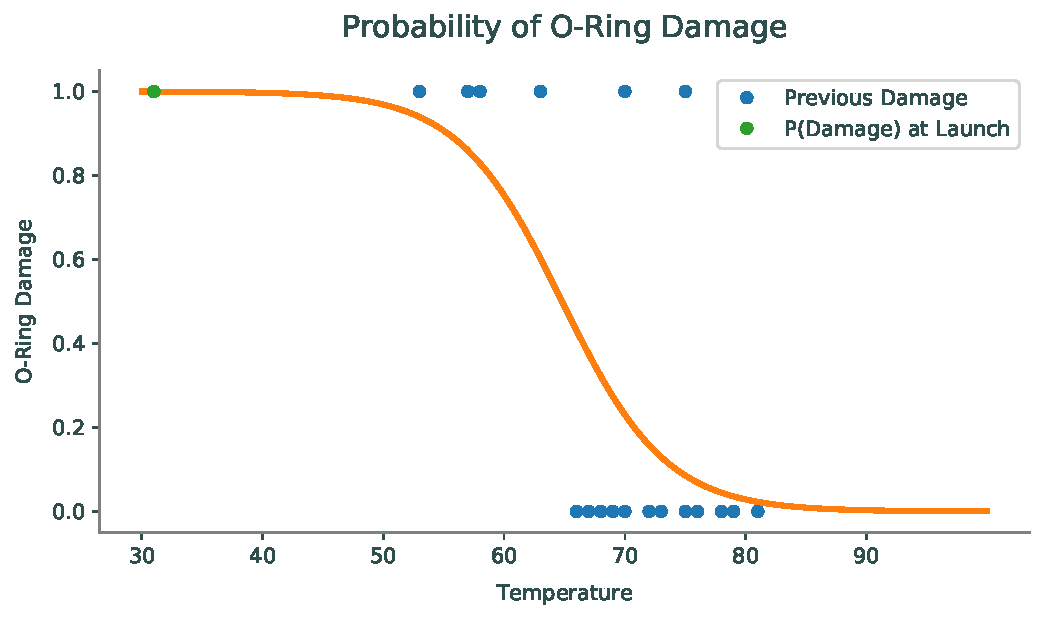
\includegraphics[width=.7\textwidth]{foundationsAppliedMathematicsLabs/Volume2/GradientMethods/figures/logreg.pdf}
    \caption{The logistic curve models the probability of O-ring damage on the Challenger shuttle. According to this model, given that the temperature was $31^\circ$ on the day of launch, the shuttle had close to $100\%$ likelihood of O-ring damage. This model had an initial guess of $1.$ and $-1$ for $\beta_0$ and $\beta_1$ respectively.}
    \label{fig:logistic_curve}
\end{figure}
\end{example}
